\documentclass{beamer}
\usepackage[utf8]{inputenc}
\usepackage{graphicx}
\usepackage{listings}
\usetheme[]{boxes}
\usecolortheme{seagull}
%\usepackage{french}
\title{Modèles et techniques en programmation parallèle hybride et multi-c\oe urs}
\author{Marc Tajchman}\institute{CEA - DEN/DM2S/STMF/LMES}

\begin{document}

\begin{frame}
\titlepage
\end{frame}

\Large
\begin{frame}
  	\frametitle{Plan (2 premières s\'eances)}
  	\tableofcontents
\end{frame}

\begin{frame}
\section{Rappels sur l'architecture mat\'erielle}
\frametitle{Rappels sur l'architecture mat\'erielle}
\textcolor{blue}{On peut voir la structure d'une machine de calcul \`a diff\'erentes \'echelles}:
\vfill

Vue globale: un ensemble de n\oe uds de calcul chacun contenant un ou plusieurs processeurs et de la m\'emoire, les n\oe uds sont connect\'es par un r\'eseau:

\vfill
\begin{center}
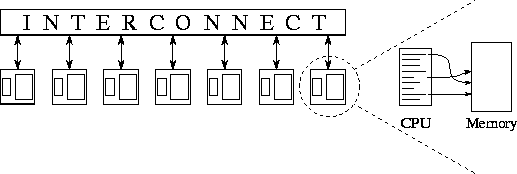
\includegraphics[scale=0.4]{img100}
\end{center}

(les machines les plus puissantes actuellement contiennent plusieurs centaines de milliers de n\oe uds)
\end{frame}

\begin{frame}
Vue interne d'un n\oe ud (variable suivant le mod\`ele de processeur et la g\'en\'eration utilis\'ee):

\begin{center}
\includegraphics[scale=0.3]{architecture2}
\end{center}

\end{frame}

\begin{frame}
Vue interne d'un c\oe ur (variable suivant le mod\`ele de processeur et la g\'en\'eration utilis\'ee):

\begin{center}
	\includegraphics[scale=0.2]{1106px-zen_block_diagram}
\end{center}

\end{frame}

\begin{frame}[fragile]
Situation actuelle (et encore pour plusieurs ann\'ees): 
\begin{quote}
	
	\vfill
	vitesse de calcul (d'un processeur)
	\vfill
	
	\begin{itemize}
		\item[$\approx$] vitesse de la m\'emoire interne (registres) du processeur
			\medskip
	        
		\item[$>$] vitesse des diff\'erentes m\'emoires cache, interm\'ediaires entre le processeur et la m\'emoire centrale du n\oe ud (vitesse L1 $>$ L2 $>$ L3, taille L1 $<$ L2 $<$ L3)
			\medskip
			
		\item[$\gg$] vitesse de la m\'emoire centrale d'un n\oe ud
			\medskip
			
		\item[$\gg$] vitesse du r\'eseau qui connecte les n\oe uds
	\end{itemize}


\end{quote}

\end{frame}

\begin{frame}[fragile]
Fonctionnement :

\begin{itemize}
	\item Les donn\'ees sont envoy\'ees dans les registres du processeur qui va les utiliser, en laissant des copies dans les diff\'erents niveaux de cache de ce processeur. 
	\vfill
	
	\item Les zones m\'emoires sont copi\'ees par bloc entre la m\'emoire centrale et les m\'emoires cache. Donc si une donn\'ee est proche d'une autre qui vient d'\^etre utilis\'ee, elle a peut-\^etre d\'ej\`a \'et\'e copi\'ee (et l'utilisation de cette 2nde donn\'ee est plus rapide)	
\end{itemize}
	\vfill
\end{frame}

\begin{frame}[fragile]
	
\begin{itemize}
	\item Si une donn\'ee est utilis\'ee $n$ fois par le m\^eme processeur dans des instructions proches, les $n-1$ derni\`eres utilisations seront plus rapides (parce que la donn\'ee sera peut-\^etre encore dans une m\'emoire cache).
\vfill

	\item Si un processeur a modifi\'e une donn\'ee dans une de ses m\'emoires, il faut r\'epercuter cette modification dans les diff\'erentes copies de cette donn\'ee.
	\vfill
\end{itemize}
	\vfill

{\bf Cette gestion peut repr\'esenter une partie im\-por\-tante du temps d'ex\'ecution (pour assurer la coh\'erence des diff\'erentes parties de la m\'emoire et leurs mises \`a jour correctes).}
	\vfill


\end{frame}

\begin{frame}[fragile]

\bf
\textcolor{blue}{Pour obtenir un code efficace (en temps d'ex\'ecution), il faut:}

\begin{itemize}
	\item utiliser les algorithmes les plus efficaces possible (pas couvert par ce cours)
	
	\item organiser le placement des donn\'ees (am\'eliorer la localit\'e spatiale)
	
	\item organiser la s\'equence d'instructions (am\'eliorer la localit\'e temporelle)

	\item \'ecrire les instructions pour qu'elles soient les plus rapides (utilisation du // interne des processeurs, \'eviter si possible les tests)
\end{itemize}
\end{frame}

\begin{frame}
\section{Programmation s\'equentielle efficace}
\frametitle{Programmation s\'equentielle efficace}
\end{frame}

\begin{frame}
\frametitle{Localit\'e spatiale}
Règle: autant que possible, utiliser des zones m\'emoires proches les unes des autres dans une s\'equence d'instructions

\vfill
But: r\'eduire la fr\'equence de transferts m\'emoire centrale - m\'emoire cache

\vfill
Exemple: voir TP 1
\end{frame}

\begin{frame}
\frametitle{Localit\'e temporelle}
Règle: autant que possible, pour une zone m\'emoire, les instructions qui l'utilisent doivent s'ex\'ecuter de façon rapproch\'ee

\vfill
But: r\'eduire la fr\'equence de transferts m\'emoire centrale - m\'emoire cache
\vfill
Exemple: voir TP 1
\end{frame}

\begin{frame}[fragile]
\frametitle{Utilisation du // interne au processeur}
Règle: essayer de rassembler plusieurs instructions simples en une seule (quand cela a un sens), essayer d'\'eviter les tests

\bigskip
But: utiliser la pr\'esence \'eventuelle de plusieurs unit\'es de calcul dans le processeur, simplifier le travail du processeur.

\end{frame}

\begin{frame}[fragile]
Exemple: remplacer
\begin{lstlisting}
for (i=0; i<n; i++) {
  u[i] = u0[i];
  if (terme1) u[i] += a*v[i];
  if (terme2) u[i] += b*w[i];
}
\end{lstlisting}

par:
\begin{lstlisting}
if (terme1) aa = a; else aa = 0.0;
if (terme2) bb = b; else bb = 0.0;
for (i=0; i<n; i++) {
   u[i] = u0[i] + aa*v[i] + bb*w[i];
}
\end{lstlisting}

\end{frame}

\begin{frame}
\section{Rappels de programmation parallèle}
\frametitle{Rappels de programmation parallèle: notions}
Points abord\'es
\begin{itemize}
\item thread - process
\item m\'emoire distribu\'ee ou partag\'ee
\end{itemize}
\end{frame}

\begin{frame}
	\subsection{Processes}
\end{frame}

\begin{frame}
	\subsection{M\'emoire partag\'ee}
\end{frame}

%\begin{frame}
%\subsection{M\'emoire partag\'ee}
%\frametitle{Rappels de programmation parallèle: m\'emoire partag\'ee}
%Points abord\'es
%\begin{itemize}
%\item Modèle d'architecture mat\'erielle
%\item Principes d'optimisation
%\item Cas classique : OpenMP, pthreads
%\item Autres
%\end{itemize}
%\end{frame}
%
%\begin{frame}
%\subsection{M\'emoire distribu\'ee}
%\frametitle{Rappels de programmation parallèle: m\'emoire distribu\'ee}
%Points abord\'es
%\begin{itemize}
%\item Modèle d'architecture mat\'erielle
%\item Principes d'optimisation
%\item Cas classique : MPI
%\item Autres
%\end{itemize}
%\end{frame}
%
%\begin{frame}
%\section{Programmation parallèle hybride}
%\frametitle{Programmation parallèle hybride \hbox{(4 s\'eances)}}
%Points abord\'es
%\begin{itemize}
%\item Coexistence 
%\item Modèles d'hybridation
%\item Cas classique : MPI - OpenMP
%\item Exemples
%\item Autres modèles (e.g. MPI+X, PGAS)
%\end{itemize}
%\end{frame}
%
%\begin{frame}
%\section{Examen}
%\frametitle{Examen \hbox{(1 s\'eance)}}
%\end{frame}

\end{document}
